
%\begin{figure}[tbp]
%\centering
%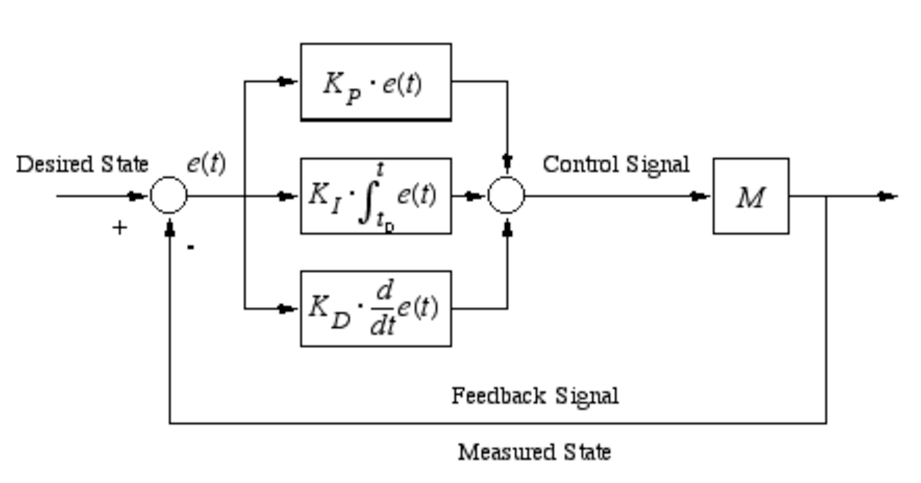
\includegraphics[width=0.5\textwidth]{images/pid.pdf}
%\caption{\label{pid-controller} PID controller}
%\end{figure}

\begin{equation}\label{pid-function}
u(t) = K_{P} e(t) + K_{I} \int_0^t e(t)\,dt + K_{D} \frac{d e(t)}{dt}
\end{equation}

\section{Introduction}\label{section_one}
Each of the three aspects of the controller represents a separate property of the error being computed. The proportional component represents the current error of the system. It is multiplied by a proportional constant and produces a value that defines the amount of response to a change in the system. Increasing the proportional component’s representation by increasing the proportional constant will create more of a response to some deviation from the desired state, however setting this constant too high can cause the system to become unstable in its attempts to adapt and too low can result in a high error to output ratio, creating insufficient attempts to reach the desired state. The integral component calculates the sum of the error of the system as time progresses. Similar to the proportional term, it is affected by an integral constant that may be adjusted to increase or decrease its contribution to the overall function. The integral component is especially useful for the PID controller as its output value relies on the previous error of the system and (in theory) maintains a decreasing but constant error that is required to drive the process, however, this creates an infinite overshooting of the desired state from the actual state of the function. Finally, the derivative component measures the slope of the change in error over time and uses this value to predict the response needed to correct the error. It is multiplied by a derivative constant that defines the magnitude of contribution by the derivative component to the overall function. In essence the derivative component determines the rate of adjustment to the error in the system and is effective at reducing the overshooting issue caused by the integral component. Unfortunately the derivative component amplifies noise in the error which can be problematic if the derivative constant is large. 


